This present section describes how the design challenges were solved in this project with respect to the serial implementation. Methods and procedures are explained in detail throughout this chapter as well.

    \section{K-Means algorithm for hyperspectral images}
    
    
    In the field of image processing, namely hyperspectral image, the clustering algorithm called K-Means is described as follows:
    
     First, K centroids are defined, one for each cluster (K number of clusters). After initializing these variables, a first grouping is implemented as the distance of each point to the centroids. Each point is identified with a cluster represented by the nearest centroid. A centroid represents the center of a cluster, in order to find it, an average of the data is performed, this refers to the means in the K-Means algorithm. This process is perform iteratively until the difference between centroids of two consecutive iterations is either smaller than a specified error or the maximum fixed number of iterations is reached. 
    
    
    The purpose of executing the processing tool chain during surgery is to define the tumour borders with precision. K-means is the algorithm that best meets this need since the major role is separate clearly different areas of the hyperspectral image. 
    
 For hyperspectral data, the classifier can be used to find spectral classes in a multiband image without assigned values from the data provider. The clustering treats unsupervised data by providing access to the tools to learn the classification from the data itself to create clusters that group the data based on the desired classification\cite{kushi2012american}.
  
 	It should be noted that in contrast with all other algorithms (PCA, SVM and KNN), K-Means does not need prior knowledge of the data; therefore, it does not have a number of fixed steps. Furthermore,data are put together in terms of feature similarity. 
 	
 
 
    \subsection{Analysis of the pseudo-code}
    
The pseudo-code described hereafter (algorithm 1), it has been taken from \cite{torti2018paralle}, where $\gamma$ indicates a hyperspectral image that consists of N pixels and L bands. Therefore, a hyperspectral image is a matrix with size $NxL$. The parameters to be set when it comes to execute the algorithm are as follows: 
\begin{itemize}
\item K which corresponds with the number of clusters to use.
\item $Min\_error$ related to the minimum error allowed.
\item $Max\_iter$ are the maximum number of iterations which are executed.
\end{itemize}

 \begin{figure}[H]
        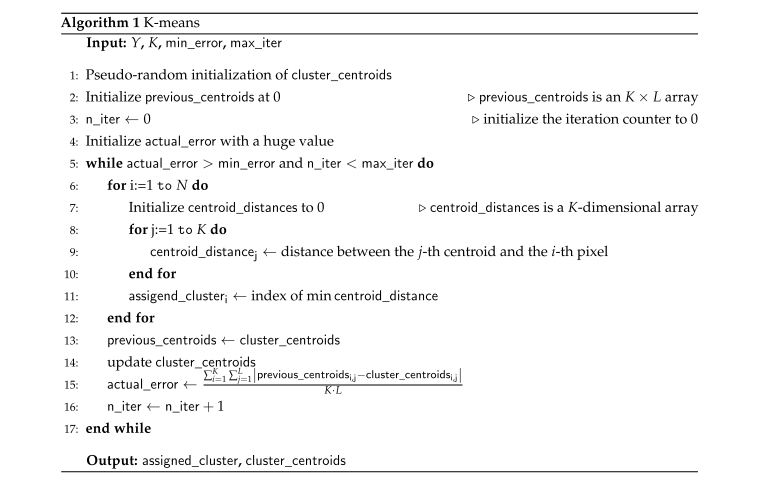
\includegraphics[scale=0.8]{pseudocode.png} 
        \centering   
        \caption{Pseudo-code of the K-means   \cite{torti2018paralle}}        
        \label{fig:systemArch}
    \end{figure}

The k-means algorithm generates different results. On one hand, a $KxL$ array including the centroids, which is called $cluster\_centroids$ and an $N-dimensional$ array which has the label of the cluster assigned to each pixel, this parameter, by contrast, it is called $assigned\_cluster$.

The K-means clustering algorithm is analysed in detail line by line. First,in lines 1 and 2 the initialization of the variables is perform. Namely,
$cluster\_centroids$ is initialized with K different hyperspectral pixels pseudo-randomly taken from the input image $\gamma$.

 The variable $actual\_error$ is initialized with a great value to make sure that the main loop is executed at least one time.
 
 As can be seen in the figure above, there are two iterative loops (from lines 6 to 12), the inner one is executed K times which are the number of clusters, and the external one iterates over the number of pixels N, instead. 
 
  A temporal array determined by $centroid\_distances$ is set to 0 and it stores the distances between each pixel and the centroids. Spectral Angle (SA) formula is used in order to calculate the measured distance between them.
  
  This Spectral Angle is defined as: 
 
   \begin{figure}[H]
        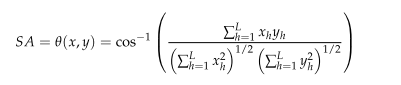
\includegraphics[scale=0.8]{Spectralformula.png} 
        \centering  
        \caption{Spectral Angle formula\cite{torti2018paralle}}          
        \label{fig:systemArch}
    \end{figure}
   
 	This formula results in spectral vectors determined by x and y. The variables $x_h$ and $y_h$ are the response of the h-th band of x and y and they go from 1 to L bands.
  
  Once this step has been executed, the label assigned to each pixel corresponds to the group represented by the centroid with the minimum SA value. This step is performed for each pixel. 

After these steps,the array $previous\_centroids$ stores the centroids with the SAs computation, and subsequently, the centroids are updated by calculating the mean value, for each band, of the pixels belonging to the group or cluster. In order to compute the error, $previous\_centroids$ and the updated centroids already calculated, are used for calculating the variation. This value represents how different they are among them, or, how much they have varied in each iteration. In addition, it is used as a stop condition when this difference is smaller than a fixed threshold ($actual\_error)$. The number of iterations is increased in each iteration, and when it reaches a value (threshold) which has been set previously,the algorithm is no longer executed. 

     \subsection{C serial code profiling}
     
	As was mentioned earlier, the C serial code has been provided by Universidad de Las Palmas de Gran Canaria.  This algorithm has been analysed in detail in order to do a  first approach of how it works internally and how each function was implemented, and then be able to parallelize it. A dataset of real HS images is used for the processing toolchain. Before executing this algorithm, certain parameters may be set, these parameters are as follows:
	
	$$K=24$$
	$$min\_error=1\mathrm{e}{-3}$$
	$$max\_error=50 \thinspace iterations$$
	
	All these parameters have been taken from \cite{torti2018paralle}. The K value was set during the development of the HS brain cancer algorithm illustrated in \cite{fabelo2018spatio}.If this configuration is set, the algorithm never reached the maximum number of iterations established.
	
	It should be noted that a function in C has been created by each process described previously. As the purpose of this research work is to parallelize a clustering algorithm, the C serial code has to be analysed in depth in order to study the heaviest part and the bottlenecks of the code which slow down the algorithm and does not allow to approach real time, which is crucial for neurosurgeons during surgery.
	
	The heaviest part of the code is undoubtedly the computation of distances,as was mentioned earlier, is the spectral angle between each hyperspectral pixel and the centroids. The time invested in the computation of the distance is approximately 26 seconds (based on the serial implementation), which along with the other functions executed inside the loop, take the 94$\%$ and $98\%$ of the time for the smallest and the biggest image according to this paper \cite{torti2018paralle}.
	
	Furthermore, initialization functions such as initialization of the error and initializaton of $cluster\_centroids$ are not parallelized since they are executed just one time in the beginning and they are not a point for consideration. 
	
	
	 \subsection{K-means in PREESM}
	 
	 The algorithm has been first implemented using $\pi SDF$ dataflow model in PREESM in order to ensures consistency and schedulability and then parallelised
	 	 
	As was explained earlier,the  $\pi SDF$ MoC is a generalization of the SDF MoC.In addition to the actors and FIFOs of the SDF semantics, the  $\pi SDF$ semantics has a set of parameters and parameter dependencies that can be used to reconfigure the production and consumption token rates of actors. Furthermore, the  $\pi SDF$ semantics has a hierarchy mechanism that enables the composition of graphs by using a $\pi    SDF$ sub-graph as a specification of the internal behaviour of an actor.
	
	First of all, the algorithm has been divided into different hierarchies in order to create independent graphs that isolate themselves from each other. Its behaviour (the instantiated ones) may not be modified by its parent graph.
	
	As this kind of model allows to create different hierarchies, a top diagram is first created. This hierarchy includes three main actors known as, "read parameters", "kmeans cluster" and "write parameters" which are explained in detail as follows:
	
	\textbf{Read parameters's actor}: A whole hyperspectral image is read and stored by this actor, from either a binary file or txt file in order to process it. Each token corresponds to a pixel in a particular band.
	 Furthermore, this actor reads a parameter called par which is the minimum error allowed.
\par
	\setlength\parindent{24pt}\textbf{Kmeans cluster}: A whole image is processed by one firing of kmeans cluster actor. This actor is refined by several actors such as initialize cluster, initialize error and kmeans function. Kmeans function actor is a hierarchical actor defined by the subgraph  formed by actors loop, compute error, compute distance and update centroids. \par
	\setlength\parindent{24pt}\textbf{Write results's actor}: This actor converts results to a image. The result is a clustered hyperspectral image.
	
	
	 \begin{figure}[H]
        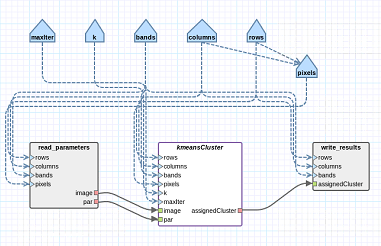
\includegraphics[scale=1.2]{top_diagram.png} 
        \centering 
        \caption{Top PiSDF graph}         
        \label{fig:systemArch}
    \end{figure}
	
	 
KmeansCluster's actor is a hierarchical actor formed by initialize cluster,initialize error and kmeansfunction. A detailed explanation is given hereunder:


\setlength\parindent{24pt}\textbf{Initialize cluster centroids}: This actor assigns an initial value to the centroids: k random non-repeated numbers are taken as indices; 
pixels of the provided set of images corresponding to these indices are the first centroids of the clusters.

\setlength\parindent{24pt}\textbf{Initialize error}: This actor calculates error between current and previous centroids. It should be noted that the error is the mean of the absolute value of the member-to-member difference of the two vectors.

\setlength\parindent{24pt}\textbf{Kmeansfunction}: This is a hierarchical actor set by loop, compute error, compute distance and update centroids actors. They will be explained later.

Finally, the deeper sub graph consists of various actors called loop, compute error, compute distance and update centroids.

\setlength\parindent{24pt}\textbf{Loop}: This actor allows create an iterative loop among actors. Actor loop is used to set the number N of iterations of the for loop.

\setlength\parindent{24pt}\textbf{Compute error}: This actor has the same behavior as the initialize error one explained earlier.

\setlength\parindent{24pt}\textbf{Compute distance}: This actor calculates the distance between each pixel and the centroids of the clusters. Each pixel is assigned to the nearest cluster. The spectral angle is used for computing the distance.

\setlength\parindent{24pt}\textbf{Update centroids}: This actor updates the centroids. In order to get an updated version of the centroids, they are calculated as mean of the elements of the cluster.


   Before starting parallelizing, the whole $\pi SDF$ graph has been tested with the hyperspectral dataset already used for serial code. The obtained clustering is the same as it was obtained in the serial implementation. This has been proven setting a fixed value in the initialization of the cluster centroids (the first cluster centroids are usually selected randomly) and analysing if the image obtained is equal to the achieved by the serial code. The parallelization of the algorithm is performed since the result turned out to be equal to the serial implementation.




	 
	
	
	
	

